\chapter{I\textsuperscript{2}C sučelje}

Za konfiguraciju kamere Arducam 5MP Mini Plus  PDH računalo koristi I\textsuperscript{2}C (engl. \textit{Inter-Integrated Circuit}) komunikaciju. S obzirom na to da se za razvoj programske potpore PDH računala koriste \textit{Low-Layer} biblioteke, potrebno je razumijevanje načina rada I\textsuperscript{2}C periferije odabranog mikrokontrolera kako bi se ispravno implementirali upravljački programi. U nastavku slijedi općeniti opis I\textsuperscript{2}C protokola kao i razlike između I\textsuperscript{2}C periferijski sklopova na prethodno korištenom (STM32F407VGT6) i trenutačnom (STM32L471VGT6) mikrokontroleru.

\section{I\textsuperscript{2}C protokol}

I\textsuperscript{2}C je jednostavna dvosmjerna sinkrona serijska sabirnica razvijena od strane \textit{Philips Semiconductors} (sada \textit{NXP Semiconductors}) 1982. godine \cite{i2c_wikipedia}. Koristi dvije linije:
\begin{itemize}
	\item serijska podatkovna linija (SDA, \textit{Serial Data Line}),
	\item serijska taktna linija (SCL, \textit{Serial Clock Line}).
\end{itemize}
Obje linije su pritegnute na visoku logičku razinu preko \textit{pull-up} otpornika. Moguće brzine prijenosa su:
\begin{itemize}
	\item do 100 kbit/s u \textit{Standard-mode} načinu rada, 
	\item do 400 kbit/s u \textit{Fast-mode} načinu rada,
	\item do 1 Mbit/s u \textit{Fast-mode Plus} načinu rada,
	\item do 3.4 Mbit/s u \textit{High-speed} načinu rada.
\end{itemize}
Navedene brzine se koriste kod dvosmjernog prijenosa, a moguća je i brzina do 5 Mbit/s u jednosmjernom prijenosu. Više uređaja se može spojiti na jednu sabirnicu, a svaki uređaj je prepoznatljiv po svojoj jedinstvenoj adresi i može se ponašati kao prijamnik ili odašiljač, ovisno o funkciji uređaja \cite{i2c_manual}. Protokol najčešće, a tako i u ovom slučaju, koristi 7-bitno adresiranje, a moguće je i korištenje 10-bitnog adresiranja. Osim konfiguracije prijamnika i odašiljača, uređaj također može biti \textit{master} uređaj ili \textit{slave} uređaj tijekom prijenosa podataka. \textit{Master} uređaj je uređaj koji inicijalizira prijenos podataka na sabirnici i generira signal takta kako bi omogućio prijenos. U tom trenutku, bilo koji uređaj koji je adresiran smatra se \textit{slave} uređajem.

Na I\textsuperscript{2}C sabirnicu se također može spojiti više \textit{master} uređaja, a primjer jednog takvog spoja sa dva mikrokontrolera dan je na slici \ref{fig:i2c_primjer_1}.
\begin{figure}[hp]
	\centering
	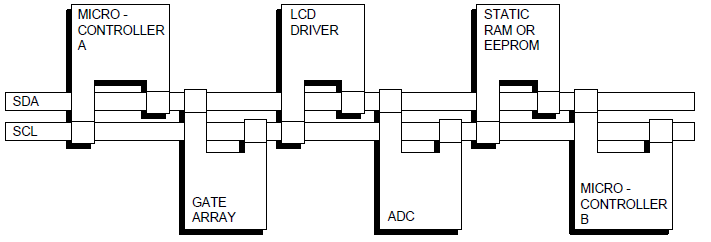
\includegraphics[width=\textwidth]{i2c_primjer_1.PNG}
	\caption{Primjer I\textsuperscript{2}C sabirnice sa spojena dva
	mikrokontrolera \cite{i2c_manual}}
	\label{fig:i2c_primjer_1}
\end{figure}
Prijenos podataka bi možda mogao izgledati ovako:
\begin{enumerate}
	\item Mikrokontroler A želi poslati podatke mikrokontroleru B:
	\begin{itemize}
		\item mikrokontroler A (\textit{master} uređaj) adresira mikrokontroler B (\textit{slave} uređaj)
		\item mikrokontroler A (\textit{master}-odašiljač) šalje podatke mikrokontroleru B (\textit{slave} uređaj-prijamnik)
		\item mikrokontroler A prekida prijenos
	\end{itemize}
	\item Mikrokontroler A želi primiti podatke sa mikrokontrolera B:
		\begin{itemize}
		\item mikrokontroler A (\textit{master} uređaj) adresira mikrokontroler B (\textit{slave})
		\item mikrokontroler A (\textit{master}-prijamnik) prima podtke sa mikrokontrolera B (\textit{slave}-odašiljač)
		\item mikroknotroler A prekida prijenos.
	\end{itemize}
\end{enumerate}
U svakom od navedenih slučajeva mikrokontroler A je generirao takt i prekidao prijenos. Kod prijenosa podataka na I\textsuperscript{2}C sabirnici, \textit{master} uređaj uvijek generira signal takta. U ovom radu korišten je samo jedan mikrokontroler, odnosno \textit{master} uređaj, pa će se u daljnjem tekstu podrazumijevati samo taj slučaj.

\subsection{Opis komunikacije i vremenski dijagram}
I\textsuperscript{2}C komunikacija započinje sa \textit{start} simbolom i završava sa \textit{stop} simbolom. Komunikacijom se može čitati ili pisati ovisno o R/W bitu u adresi. Struktura adresiranja kod 7-bitne adrese je prikazana u tablici \ref{Tab:i2c_seven_bit_adressing}.
\begin{center}
	\begin{table}[H]
		\centering
		\begin{tabular}{ | c | c | c | c | c | c | c | c | c | }
			\hline
			& \multicolumn{7}{|c|}{Adresno polje} & R\textbackslash W \\
			\hline
			Pozicija bita u bajtu & 7 & 6 & 5 & 4 & 3 & 2 & 1 & 0 \\
			\hline
			Značenje & MSB & \multicolumn{5}{|c|}{} & LSB & 1=READ, 0=WRITE \\
			\hline
		\end{tabular}
		\caption{Struktura adresiranja kod 7-bitne adrese \cite{i2c_wikipedia}}
		\label{Tab:i2c_seven_bit_adressing}
	\end{table}
\end{center}
Iz tablice je vidljivo da najmanje značajan bit označava želi li se podatak čitati ili pisati.

Imajući na umu izgled adresnog bajta, vremenski dijagram tipčne I\textsuperscript{2}C komunikacije prikazan je na slici \ref{fig:i2c_timing_diagram}.
\begin{figure}[hp]
	\centering
	
\includegraphics[width=\textwidth]{I2C_data_transfer.png}
	\caption{Vremenski dijagram I\textsuperscript{2}C komunikacije
	\cite{i2c_wikipedia}}
	\label{fig:i2c_timing_diagram}
\end{figure}
\begin{itemize}
	\item Prijenos podataka se inicijalizira \textit{start} uvjetom (S) tako da SDA linija prijeđe u nisku logičku razinu dok SCL linija ostaje u visokoj logičkoj razini.
	\item (Plavo područje) SCL prelazi u nisku logičku razinu i SDA postavlja prvi podatkovni bit dok je SCL u niskoj logičkoj razini.
	\item (Zeleno područje) Podaci se primaju dok SCL poraste za prvi bit (B\textsubscript{1}). Kako bi podaci bili valjani, SDA se ne smije promijeniti između rastućeg brida SCL-a i sljedećeg padajućeg brida.
	\item Postupak se ponavlja, SDA se postavlja dok je SCL u niskoj razini, a podaci se čitaju dok je SCL u visokoj razini (B\textsubscript{2} do B\textsubscript{n}).
	\item Nakon posljednjeg bita slijedi taktni impuls, tijekom kojeg SDA prelazi u nisku razinu pripremajući se za \textit{stop} uvjet.
	\item Signalizira se \textit{stop} uvjet kada SCL prijeđe u visoku logički razinu, nakon čega slijedi prelazak u visoku logičku razinu SDA signala.
	\item (Plavo područje) SCL prelazi u nisku logičku razinu i SDA postavlja
\end{itemize}
\textit{Start} i \textit{stop} uvjete uvijek generira \textit{master} uređaj. Nakon svakog bajta prijamnik šalje odašiljaču ACK bit kojim se signalizira uspješno primanje podatka, odnosno NACK bit kojim se signalizira neuspješno primanje podatka. ACK i NACK bitovi se nazivaju signalom potvrde i definiraju se na sljedeći način: odašiljač otpušta SDA liniju tijekom potvrdnog takta kako bi prijamnik mogao spustiti SDA na nisku razinu na kojoj i ostaje tijekom visoke razine takta. Ako SDA ostaje u visokoj razini tijekom devete periode takta, to predstavlja NACK (engl. \textit{Not Acknowledge}) signal, a suprotan slučaj predstavlja ACK (engl. \textit{Acknowledge}) signal. Ako je došlo do NACK signala, \textit{master} uređaj može generirati \textit{stop} uvjet kako bi prekinuo prijenos ili može ponovno generirati \textit{start} uvjet kako bi započeo novi prijenos. Vremenski dijagram cijele komunikacije s potvrdnim signalima prikazan je na slici \ref{fig:i2c_timing_diagram_transaction}.

\begin{figure}[hp]
	\centering
	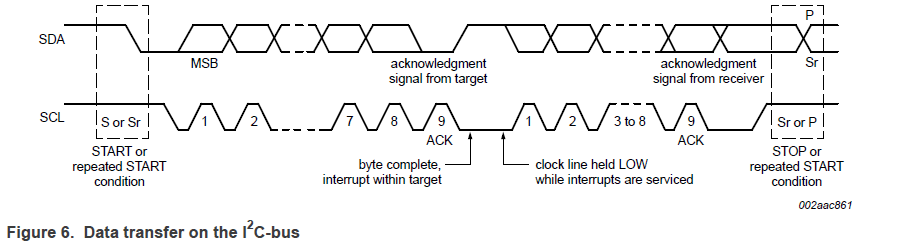
\includegraphics[width=\textwidth]{I2C_vremenski_dijagram.PNG}
	\caption{Prijenos podataka na I\textsuperscript{2}C sabirnici \cite{i2c_manual}}
	\label{fig:i2c_timing_diagram_transaction}
\end{figure}

\section{Razlika I\textsuperscript{2}C periferije na STM32L471VGT6 i \newline STM32F407VGT6 mikrokontrolerima}

Tijekom prijenosa koda sa starog mikrokontrolera na novi, primjećeno je da postoji razlika između struktura I\textsuperscript{2}C periferija. Točnije, postoji razlika između registarskih mapa na dvama periferijama, koje su vidljive usporedbom tablica \ref{Tab:l471_i2c_register_map} i \ref{Tab:f407_i2c_register_map} (\textit{napomena}: u tablicama nisu prikazani svi registri, jer se neki registri niti ne koriste, ili se koriste samo tijekom konfiguracije periferija. Za puni prikaz tablica treba provijeriti dokumentacije mikrokontrolera \cite{f407_manual}, \citep{l471_manual}).

\begin{table}[H]
	\resizebox{\textwidth}{!}{%
	\begin{tabular}{|c|c|c|l|l|l|l|l|l|l|l|l|l|l|l|l|l|l|l|l|l|l|l|l|l|l|l|l|l|l|l|l|l|l|}
		\hline
		\textbf{Offset} & \textbf{\begin{tabular}[c]{@{}c@{}}Register\\ name\end{tabular}} & \rotbf{31} & \rotbf{30} & \rotbf{29} & \rotbf{28} & \rotbf{27} & \rotbf{26} & \rotbf{25} & \rotbf{24} & \rotbf{23} & \rotbf{22} & \rotbf{21} & \rotbf{20} & \rotbf{19} & \rotbf{18} & \rotbf{17} & \rotbf{16} & \rotbf{15} & \rotbf{14} & \rotbf{13} & \rotbf{12} & \rotbf{11} & \rotbf{10} & \rotbf{9} & \rotbf{8} & \rotbf{7} & \rotbf{6} & \rotbf{5} & \rotbf{4} & \rotbf{3} & \rotbf{2} & \rotbf{1} & \rotbf{0} \\
		\hline
		\multirow{2}{*}{0x0} & I2C\_CR1 & \multicolumn{8}{c|}{Res.} & \rot{PECEN} & \rot{ALERTEN} & \rot{SMBDEN} & \rot{SMBHEN} & \rot{GCEN} & \rot{WUPEN} & \rot{NOSTRETCH} & \rot{SBC} & \rot{RXDMAEN} & \rot{TXDMAEN} & \rot{Res.} & \rot{ANFOFF} & \multicolumn{4}{c|}{DNF[3:0]} & \rot{ERRIE} & \rot{TCIE} & \rot{STOPIE} & \rot{NACKIE} & \rot{ADDRIE} & \rot{RXIE} & \rot{TXIE} & \rot{PE} \\
		\cline{2-34}
		& Reset value & & & & & & & & & 0 & 0 & 0 & 0 & 0 & 0 & 0 & 0 & 0 & 0 & & 0 & 0 & 0 & 0 & 0 & 0 & 0 & 0 & 0 & 0 & 0 & 0 & 0 \\
		\hline
		\multirow{2}{*}{0x4} & I2C\_CR2 & \multicolumn{5}{c|}{Res.} & \rot{PECBYTE} & \rot{AUTOEND} & \rot{RELOAD} & \multicolumn{8}{c|}{NBYTES[7:0]} & \rot{NACK} & \rot{STOP} & \rot{START} & \rot{HEAD10R} & \rot{ADD10} & \rot{RD\_WRN} & \multicolumn{10}{c|}{SADD[9:0]} \\
		\cline{2-34}
		& Reset value & & & & & & 0 & 0 & 0 & 0 & 0 & 0 & 0 & 0 & 0 & 0 & 0 & 0 & 0 & 0 & 0 & 0 & 0 & 0 & 0 & 0 & 0 & 0 & 0 & 0 & 0 & 0 & 0 \\
		\hline
		\multirow{2}{*}{0x18} & I2C\_ISR & \multicolumn{8}{c|}{Res.} & \multicolumn{7}{c|}{ADDCODE[6:0]} & \rot{DIR} & \rot{BUSY} & \rot{Res.} & \rot{ALERT} & \rot{TIMEOUT} & \rot{PECERR} & \rot{OVR} & \rot{ARLO} & \rot{BERR} & \rot{TCR} & \rot{TC} & \rot{STOPF} & \rot{NACKF} & \rot{ADDR} & \rot{RXNE} & \rot{TXIS} & \rot{TXE} \\
		\cline{2-34}
		& Reset value & & & & & & & & & 0 & 0 & 0 & 0 & 0 & 0 & 0 & 0 & 0 & & 0 & 0 & 0 & 0 & 0 & 0 & 0 & 0 & 0 & 0 & 0 & 0 & 0 & 0 \\
		\hline
		\multirow{2}{*}{0x1C} & I2C\_ICR & \multicolumn{18}{c|}{Res.} & \rot{ALERTCF} & \rot{TIMOUTCF} & \rot{PECCF} & \rot{OVRCF} & \rot{ARLOCF} & \rot{BERRCF} & \multicolumn{2}{c|}{Res.} & \rot{STOPCF} & \rot{NACKCF	} & \rot{ADDRCF} & \multicolumn{3}{c|}{Res.} \\
		\cline{2-34}
		& Reset value & & & & & & & & & & & & & & & & & & & 0 & 0 & 0 & 0 & 0 & 0 & & & 0 & 0 & 0 & & & \\
		\hline
		\multirow{2}{*}{0x24} & I2C\_RXDR & \multicolumn{24}{c|}{Res.} & \multicolumn{8}{c|}{RXDATA[7:0]} \\
		\cline{2-34}
		& Reset value & & & & & & & & & & & & & & & & & & & & & & & & & 0 & 0 & 0 & 0 & 0 & 0 & 0 & 0 \\
		\hline
		\multirow{2}{*}{0x28} & I2C\_TXDR & \multicolumn{24}{c|}{Res.} & \multicolumn{8}{c|}{TXDATA[7:0]} \\
		\cline{2-34}
		& Reset value & & & & & & & & & & & & & & & & & & & & & & & & & 0 & 0 & 0 & 0 & 0 & 0 & 0 & 0 \\
		\hline
	\end{tabular}%
	}
	\caption{Registarska mapa I\textsuperscript{2}C periferije STM32L471VGT6 mikrokontrolera \cite{l471_manual}}
	\label{Tab:l471_i2c_register_map}
\end{table}

\begin{table}[H]
	\resizebox{\textwidth}{!}{%
	\begin{tabular}{|c|c|c|l|l|l|l|l|l|l|l|l|l|l|l|l|l|l|l|l|l|l|l|l|l|l|l|l|l|l|l|l|l|l|}
		\hline
		\textbf{Offset} & \textbf{\begin{tabular}[c]{@{}c@{}}Register\\ name\end{tabular}} & \rotbf{31} & \rotbf{30} & \rotbf{29} & \rotbf{28} & \rotbf{27} & \rotbf{26} & \rotbf{25} & \rotbf{24} & \rotbf{23} & \rotbf{22} & \rotbf{21} & \rotbf{20} & \rotbf{19} & \rotbf{18} & \rotbf{17} & \rotbf{16} & \rotbf{15} & \rotbf{14} & \rotbf{13} & \rotbf{12} & \rotbf{11} & \rotbf{10} & \rotbf{9} & \rotbf{8} & \rotbf{7} & \rotbf{6} & \rotbf{5} & \rotbf{4} & \rotbf{3} & \rotbf{2} & \rotbf{1} & \rotbf{0} \\
		\hline
		\multirow{2}{*}{0x0} & I2C\_CR1 & \multicolumn{16}{c|}{Res.} & \rot{SWRST} & \rot{Res.} & \rot{ALERT} & \rot{PEC} & \rot{POS} & \rot{ACK} & \rot{STOP} & \rot{START} & \rot{NOSTRETCH} & \rot{ENGC} & \rot{ENPEC} & \rot{ENARP} & \rot{SMBTYPE} & \rot{Res.} & \rot{SMBUS} & \rot{PE} \\
		\cline{2-34}
		& Reset value & & & & & & & & & & & & & & & & & 0 & & 0 & 0 & 0 & 0 & 0 & 0 & 0 & 0 & 0 & 0 & 0 & & 0 & 0 \\
		\hline
		\multirow{2}{*}{0x4} & I2C\_CR2 & \multicolumn{19}{c|}{Res.} & \rot{LAST} & \rot{DMAEN} & \rot{ITBUFEN} & \rot{ITEVTEN} & \rot{ITERREN} & \multicolumn{2}{c|}{Res.} & \multicolumn{6}{c|}{FREQ[5:0]} \\
		\cline{2-34}
		& Reset value & & & & & & & & & & & & & & & & & & & & 0 & 0 & 0 & 0 & 0 & & & 0 & 0 & 0 & 0 & 0 & 0 \\
		\hline
		\multirow{2}{*}{0x10} & I2C\_DR & \multicolumn{24}{c|}{Res.} & \multicolumn{8}{c|}{DR[7:0]} \\
		\cline{2-34}
		& Reset value & & & & & & & & & & & & & & & & & & & & & & & & & 0 & 0 & 0 & 0 & 0 & 0 & 0 & 0 \\
		\hline
		\multirow{2}{*}{0x14} & I2C\_SR1 & \multicolumn{16}{c|}{Res.} & \rot{SMBALERT} & \rot{TIMEOUT} & \rot{Res.} & \rot{PECERR} & \rot{OVR} & \rot{AF} & \rot{ARLO} & \rot{BERR} & \rot{TxE} & \rot{RxNE} & \rot{Res.} & \rot{STOPF} & \rot{ADD10} & \rot{BTF} & \rot{ADDR} & \rot{SB} \\
		\cline{2-34}
		& Reset value & & & & & & & & & & & & & & & & & 0 & 0 & & 0 & 0 & 0 & 0 & 0 & 0 & 0 & & 0 & 0 & 0 & 0 & 0 \\
		\hline
		\multirow{2}{*}{0x18} & I2C\_SR2 & \multicolumn{16}{c|}{Res.} & \multicolumn{8}{c|}{PEC[7:0]} & \rot{DUALF} & \rot{SMBHOST} & \rot{SMBDEFAUL} & \rot{GENCALL} & \rot{Res.} & \rot{TRA} & \rot{BUSY} & \rot{MSL} \\
		\cline{2-34}
		& Reset value & & & & & & & & & & & & & & & & & 0 & 0 & 0 & 0 & 0 & 0 & 0 & 0 & 0 & 0 & 0 & 0 & & 0 & 0 & 0 \\
		\hline
	\end{tabular}%
	}
	\caption{Registarska mapa I\textsuperscript{2}C periferije STM32F407VGT6 mikrokontrolera \cite{f407_manual}}
	\label{Tab:f407_i2c_register_map}
\end{table}

Vidljiva je razlika između količine registara, raspodjele i značenja njihovih bitova, kao i njihovih imena, što implicira različite funkcionalnosti pojedinih registara. Tako, npr. I\textsuperscript{2}C periferija kod STM32F407VGT6 sadržava 2 status registra: I2C\_SR1 i I2C\_SR2, dok kod STM32L471VGT6 postoji samo jedan status registar I2C\_ISR. Ta razlika je bitna zato što se tijekom prijenosa podataka na I\textsuperscript{2}C sabirnici trebaju provjeravati razne zastavice koje se mijenjaju tijekom komunikacije, kao što je npr. zastavica za prazni odašiljački registar (STM32F407VGT6: registar I2C\_SR1 bit 7, STM32L471VGT6: bit 0), zastavica za puni prijamnički registar (STM32F407VGT6: registar I2C\_SR1, bit 6, STM32L471VGT6: bit 2), zastavica za završetak prijenosa (STM32F407VGT6: ne postoji, STM32L471VGT6: bit 6) itd.

Vidljivo je također da kod STM32L471VGT6 postoji zastavica ADDR, koja inače kod STM32F407VGT6 signalizira uspješan primitak adrese uređaja mete, a kod \newline STM32L471VGT6 ta zastavica se koristi isključivo u \textit{slave} načinu rada, tako da ta zastavica nije bitna za ovaj projekt. Kako onda mikrokontroler zna da je poslana adresa točna? Naime, STM32L471VGT6 ima poseban registar za pohranu adrese uređaja mete, pa kada mikrokontroler pošalje \textit{start} uvjet on automatski nakon završetka \textit{start} uvjeta pošalje i adresu uređaja mete, a uspješan primitak adrese signalizira zastavica I2C\_ISR\_TXIS kod slanja podataka, odnosno I2C\_ISR\_RXNE zastavica kod primitka podataka.

Vidljive su i razlike u raspodjeli zastavica u registrima, kao i razlike u funkcijama koje zastavice signaliziraju. Inače bi te razlike stvarale probleme kod konfiguracije I\textsuperscript{2}C periferije, no, kako je tu brigu riješio kod generator ugrađen u STM32CubeIDE razvojno okruženje, nije bila posvećena pažnja tim razlikama. Način implementacije spomenutih razlika u programsku podršku opisan je u poglavlju z.